% -- Encoding UTF-8 without BOM
% -- XeLaTeX => PDF (BIBER)

\documentclass[espanol]{cv-style}     % Add 'print' as an option into the square bracket to remove colours from this template for printing. 
                                      % Add 'espanol' as an option into the square bracket to change the date format of the Last Updated Text
%\setdefaultlanguage{spanish}
%\sethyphenation[variant=spanish]{}{}  % Add words between the {} to avoid them to be cut 

\usepackage{graphicx}

\begin{document}

\header{Tom\'as }{Miguez}
\lastupdated

%----------------------------------------------------------------------------------------
% SIDEBAR SECTION  -- In the aside, each new line forces a line break
%----------------------------------------------------------------------------------------
\begin{aside}
%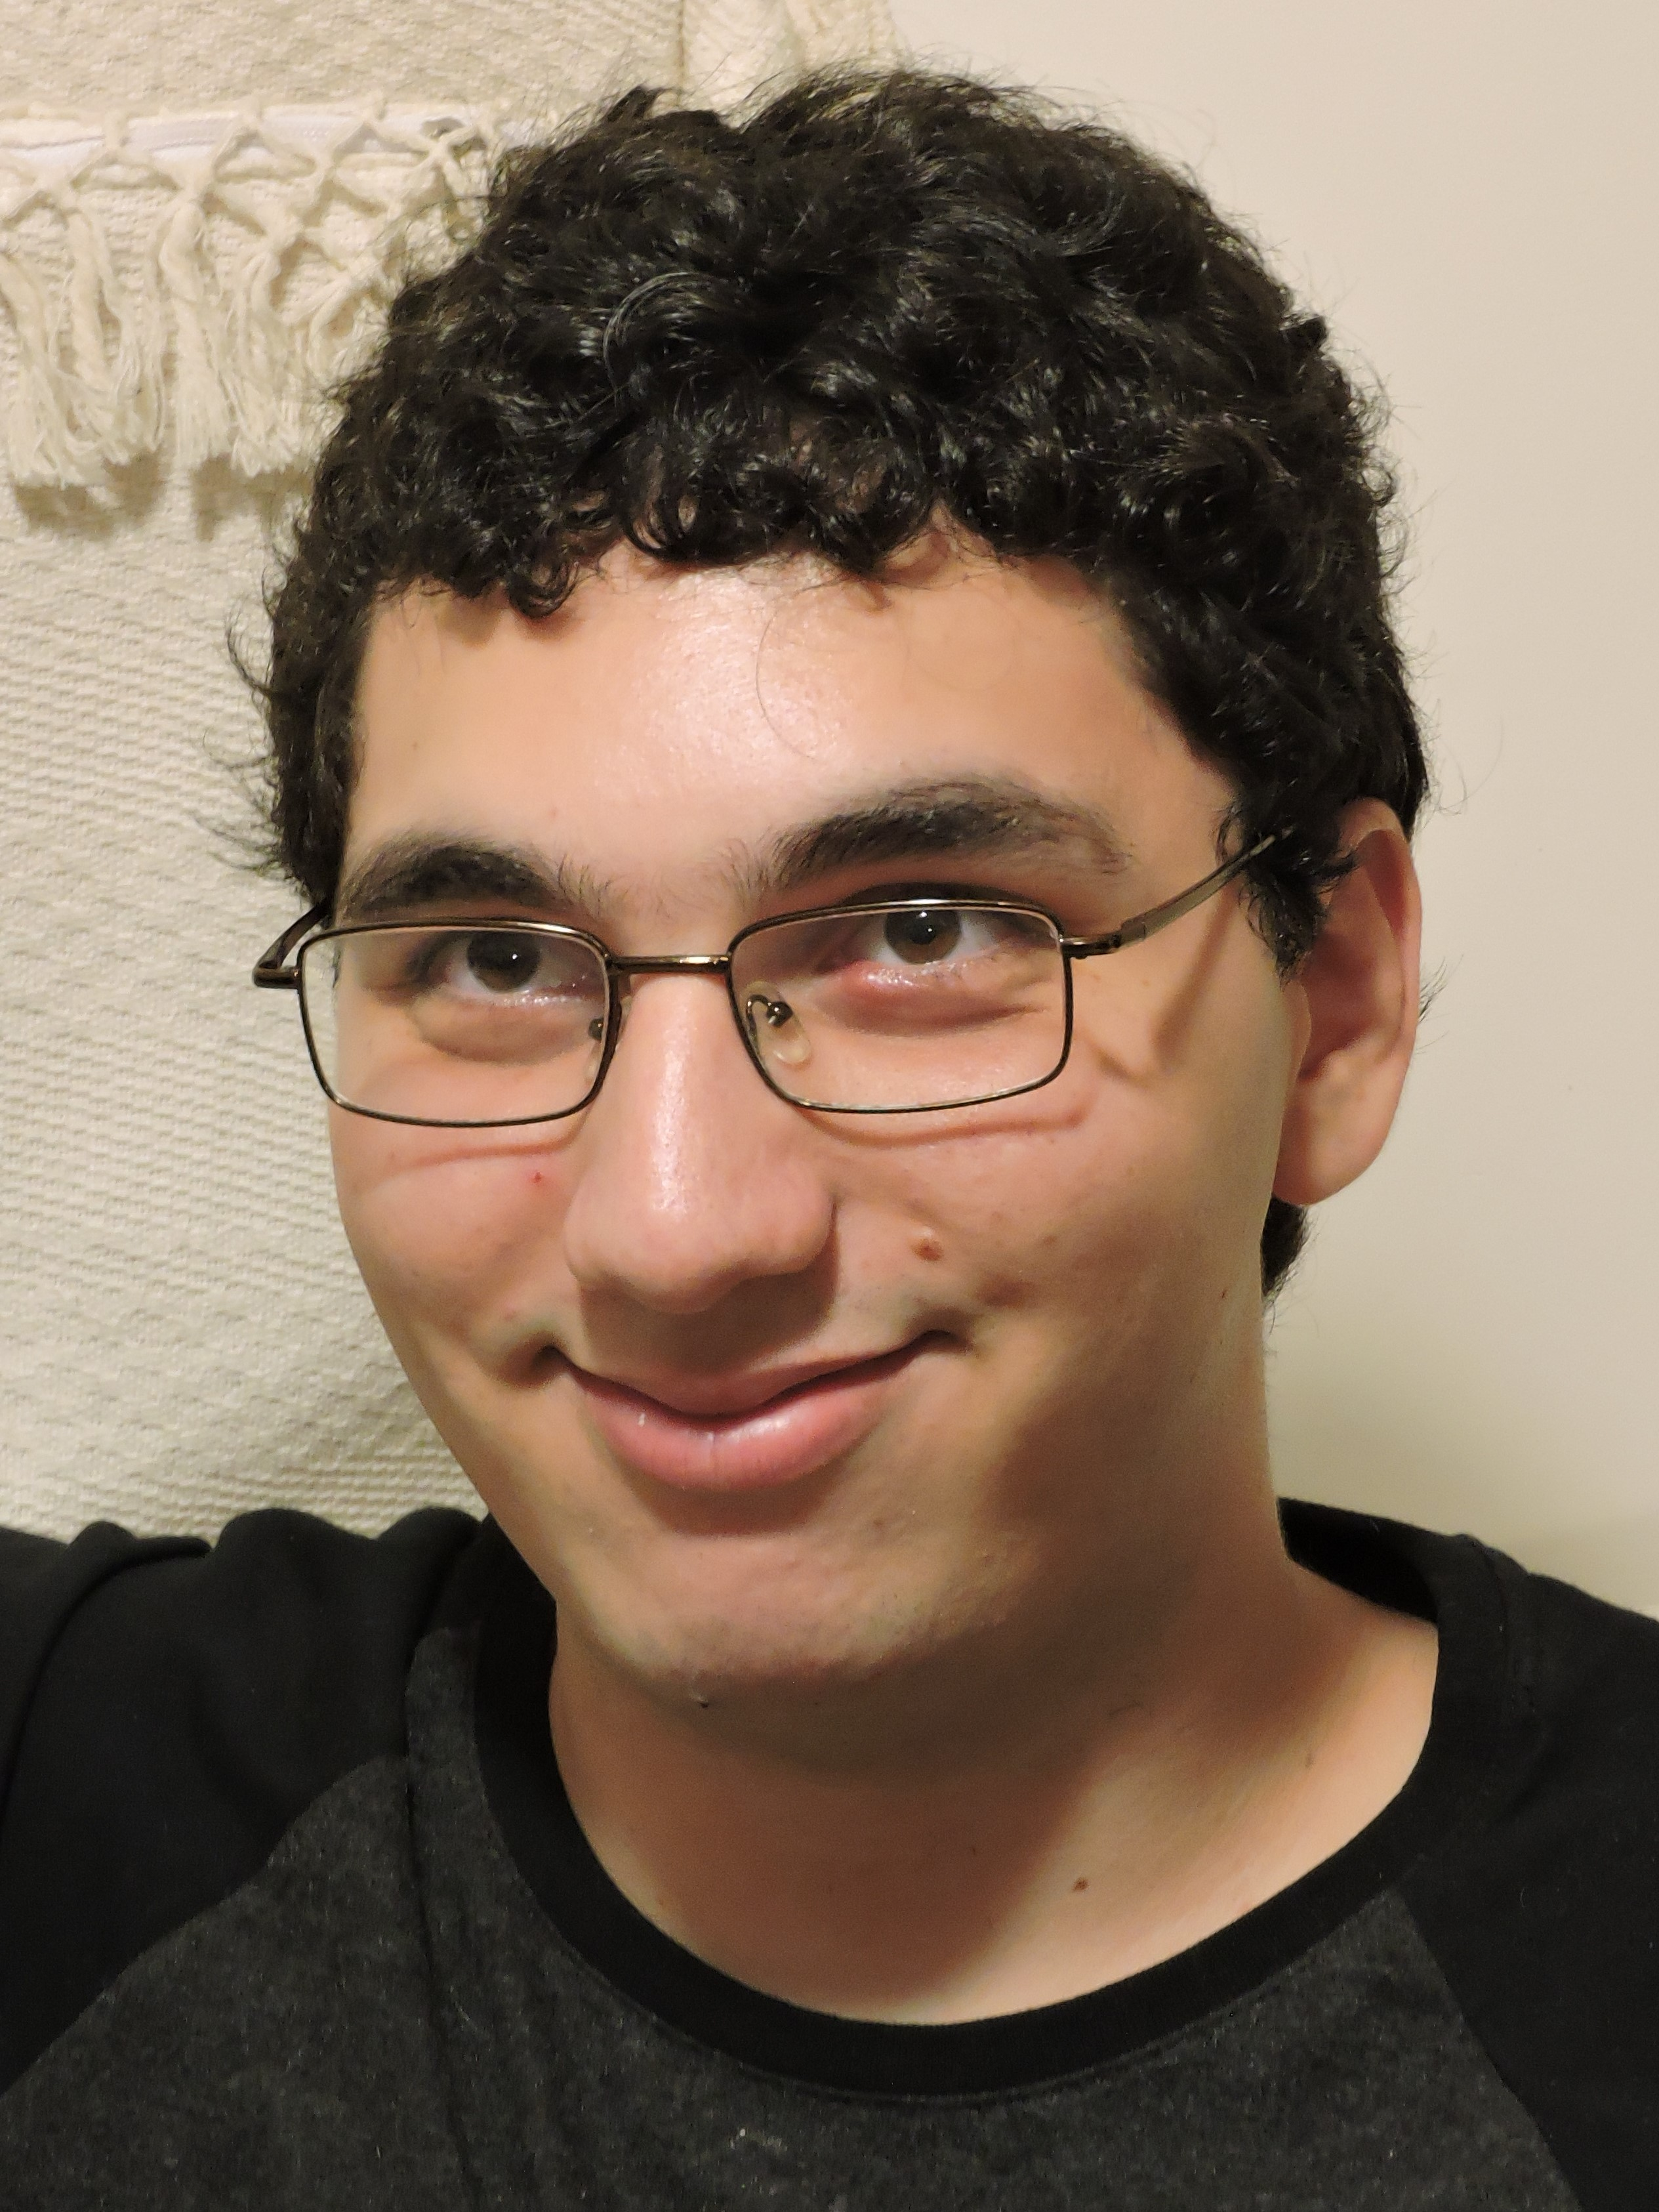
\includegraphics[width=4cm]{22}
%
\section{Datos personales}
22 años, argentino
D.N.I.: 41915119
%
\section{Contacto}
(011) 15 36453162
~
tomas.miguez@philips.edu.ar
~
Raúl Scalabrini Ortiz 2851 7B
Palermo, CABA, Argentina
%
\section{Idiomas}
Español (lengua materna),
Inglés (lectura y escritura técnica nivel avanzado, oral nivel intermedio)
%
\section{Lenguajes de programación}
%{\color{red} $\varheartsuit$} 
C++, Python
%
\section{Desarrollo web}
ASP, Bootstrap, HTML5, CSS3, JavaScript/Node.js, Apache/IIS WEB Servers
%
\section{Tecnologías miscelaneas}
Linux, GIT, SQL Server, Latex, Excel Intermedio (dinamicas, VB, Crystal reports)
%
\end{aside}
%----------------------------------------------------------------------------------------
% RESUMEN SECTION
%----------------------------------------------------------------------------------------
\vspace{0.2cm}
\section{Resumen}
  \vspace{-0.2cm}
Actualmente soy estudiante de la Facultad de Ciencias Exactas y Naturales de la UBA. Me dedico a la docencia en el área de programación y algebra y tengo experiencia en sistemas y diseño web. 
%----------------------------------------------------------------------------------------
% WORK EXPERIENCE SECTION
%----------------------------------------------------------------------------------------
\section{Experiencia}
  \vspace{-0.2cm}
\begin{entrylist}
%------------------------------------------------
\entry
  {\scalebox{.8}[1.0]{2017--Actualidad}}
  {Instituto Tecnologico Philips Argentina S.A.}
  {Ciudad Autónoma de Buenos Aires, Argentina}
  {\jobtitle{Profesor}\\
  Soy profesor del área de programación de la Escuela Philips. Las clases se dictan en C++ y cubren los fundamentos de los lenguajes de programación, tanto en el paradigma de programación estructurada como en orientada a objetos. El enfoque de las clases es resolución de problemas con la asistencia de herramientas de álgebra lineal y programación.}
%------------------------------------------ ------
\vspace{-0.3cm}
\entry
  {\scalebox{.8}[1.0]{2016--2018}}
  {Instituto Tecnológico Philips Argentina S.A.}
  {Ciudad Autónoma de Buenos Aires, Argentina}
  {\jobtitle{Técnico Sistemas}\\
     Mantenimiento de hardware y servicios web. Desarrollo web en ASP principalmente.}
%   {\jobtitle{Técnico Sistemas}\\
%     Entre mis responsabilidades en este puesto se pueden mencionar al desarrollo y mantenimiento de aplicaciones web para simplificar y agilizar distintas tareas, tanto a pedido como por propia iniciativa. Mantenimiento de la infraestructura de servidores y equipos. Asistencia al personal.
   
%     \textbf{Proyectos desarrollados:}
%     \begin{itemize}\small{
%     \item Sistema de fichada.
%     \item Carga online de calificaciones.
%     \item Sistema de marketing con integración con Facebook y WhatsApp.
%     \item Descuento por inasistencias en base a fichadas.
%     }
%   \end{itemize}}
%------------------------------------------------
\end{entrylist}
%----------------------------------------------------------------------------------------
% EDUCATION SECTION
%----------------------------------------------------------------------------------------
\section{Educación}
  \vspace{-0.2cm}
\begin{entrylist}
%------------------------------------------------
\entry
{\scalebox{.8}[1.0]{2018--Actualidad}}
{Licenciatura en Ciencias de la Computación}
{Facultad de Cs. Exactas y Naturales, UBA}
{\textbf{Promedio: 8.5}\\
\small{Materias aprobadas: CBC aprobado con promedio 8.66; Álgebra 5; Análisis Matemático 8; Algoritmos y Estructuras de Datos I 9; Algoritmos y Estructuras de Datos II 9; Probabilidad y Estadística (Final Pendiente); Sistemas Operativos I 10; Sistemas Operativos II 10; Métodos Numéricos (Final Pendiente); Teoría de las Comunicaciones / Redes (Promocionada); Ingeniería de Software I (Promocionada).\\
}}
%------------------------------------------------
\entry
{\scalebox{.8}[1.0]{2018--Actualidad}}
{Licenciatura en Ciencias Matematicas}
{Facultad de Cs. Exactas y Naturales, UBA}
{\textbf{Promedio: 8.125}\\
\small{Materias aprobadas: CBC aprobado con promedio 8.66; Álgebra 5; Análisis Matemático 8; Álgebra Lineal (Final Pendiente); Análisis II (Final Pendiente); T. Calculo avanzado.\\
}}
%------------------------------------------------
\entry
{\scalebox{.8}[1.0]{2012--2017}}
{Técnico Bilingüe Mecánico Electricista}
{Escuela Philips, Colegiales, Buenos Aires, Argentina}
{Promedio: 7.33}
%------------------------------------------------
\end{entrylist}
%----------------------------------------------------------------------------------------
% AWARDS SECTION
%----------------------------------------------------------------------------------------
\section{Extracurricular}
  \vspace{-0.2cm}
\begin{entrylist}
%------------------------------------------------
\entry
{\scalebox{.8}[1.0]{2014--2017}}
{Exámenes Internacionales de Inglés}
{}
{Cambridge English: First; Cambridge English: Advanced}
%------------------------------------------------
\end{entrylist}
  \vspace{-0.2cm}
%----------------------------------------------------------------------------------------
% INTERESTS SECTION
%----------------------------------------------------------------------------------------3
\section{Intereses}
  \vspace{-0.2cm}
\textbf{Back-end.} Sectores de análisis de datos y categorización (Machine Learning); optimización de procesos; mantenimiento de servidores y bases de datos; seguridad informática; APIs y microservicios.
%----------------------------------------------------------------------------------------
\end{document}